\documentclass[11pt,a4paper]{article}

\usepackage[T1]{fontenc}
\usepackage[utf8]{inputenc}
\usepackage{lmodern}
\usepackage[margin=2.4cm]{geometry}
\usepackage{amsmath,amssymb}
\usepackage{graphicx}
\usepackage{booktabs}
\usepackage{caption}
\usepackage{subcaption}
\usepackage{microtype}
\usepackage[numbers,sort&compress]{natbib}
\usepackage[hidelinks]{hyperref}

\captionsetup{font=small,labelfont=bf}
\graphicspath{{figures/}}
\setlength{\parskip}{0.15em}
\newcommand{\relay}{R.E.L.A.Y.}
\newcommand{\pcu}{PCU}

\title{\bfseries A Low-Cost Single-Camera Adaptive Signal Controller\\
for Heterogeneous Urban Traffic: Self-Calibrating Pressure Control\\
with Bounded Fairness and Emergency Preemption}

\author{Niraj Kafle\thanks{Kathmandu, Nepal. Correspondence: \texttt{contact.me.kafle@gmail.com}.
Source code, experiment scripts and raw result files: \url{https://github.com/kafle1/relay}.}}

\date{}

\begin{document}
\maketitle

\begin{abstract}
\noindent
Fixed-time signal plans remain the default in many South Asian cities, where traffic is
motorcycle-dominated, demand is strongly asymmetric between approaches, and the budget for inductive
loops or radar is unavailable. We present \relay, an adaptive signal controller whose only input is one
existing fixed junction camera. A single convolutional detector produces per-approach, per-class vehicle
counts, which are converted to passenger-car-unit (\pcu) demand and consumed by a queue-weighted
pressure controller in the max-pressure family. The controller adds the operational rules a deployable
signal needs and a plain argmax policy lacks: empty-phase skipping, gap-out, minimum and maximum green,
a hard anti-starvation bound, pedestrian demand treated as pressure rather than as a fixed interval, and
emergency preemption with a bounded hold. It also estimates each approach's arrival and discharge rate
from the same counts, with no site survey and no configured saturation flow, and uses those estimates for
two decisions a constant cannot make: the green is sized from Webster's cycle evaluated on the measured
degree of saturation, and a phase change is priced at the discharge its clearance interval forfeits.
We evaluate it in a seeded point-queue microsimulation against an equal-split fixed-time plan and against
a deliberately favourable reference whose cycle and splits come from Webster's formulae applied to the
true mean demand. Across 30 seeds per cell, three demand shapes and five demand levels, mean delay falls
by 28.4\% to 44.3\% against the Webster plan and by 27.9\% to 96.1\% against the equal-split plan, with
the 95th-percentile wait cut from 25.8~s to 14.5~s at 1278~veh/h. A wider robustness sweep of 72 cells,
spanning seven demand shapes, two junction topologies and loads to 2462~veh/h, beats both baselines in 71;
the exception is a single approach demanding 82\% of all green, where no cycle short enough to respect the
configured fairness bound is stable. We report one negative result: in a three-junction corridor, disabling
the downstream coupling term changes mean delay by at most 0.9\%, so the corridor gain of 44.6\% to 57.9\%
comes from local adaptivity rather than from coordination. Emergency preemption reaches green in 4.09~s on
average over 900 trials, with a measured worst case of 13.99~s against an analytical bound of 14.0~s. The
perception stack runs at a median of 38.3~ms per frame at 960~px inference on a consumer laptop, but on
motorcycle-dense footage it undercounts severely, with sampled counts rising 83\% between 640~px and
1600~px without converging. This is a simulation and real-footage feasibility study, not a field
deployment.
\end{abstract}

\noindent\textbf{Keywords:} adaptive traffic signal control; max-pressure control; computer
vision; heterogeneous traffic; emergency vehicle preemption; low-cost intelligent transport systems

\section{Introduction}

Urban signal control in low- and middle-income cities is usually performed by fixed-time plans or by
police officers operating signals manually. Both allocate green without measuring what is queued.
The consequence is visible at almost any asymmetric junction: a busy arterial approach holds a long
queue while the crossing minor street receives the green it would receive at three in the morning.
Webster's method \citep{Webster1958TrafficSignalSettings} showed that cycle length and splits should
follow demand, but a fixed plan can only follow the demand measured when the plan was designed, and
re-timing surveys are infrequent. Studies of signalised intersections in the Kathmandu valley report
saturation flows and delays that differ substantially from standard capacity guidance, attributing
the difference to the local vehicle mixture and to lane discipline
\citep{shrestha2014development,nepali2024assessment}, which is exactly the condition under which a
plan imported from a design manual performs badly.

The established remedy is a demand-responsive system such as SCOOT
\citep{Hunt1981SCOOT,Robertson1991SCOOTMethod} or SCATS \citep{Sims1980SCATS}, or an
optimisation-based controller in the OPAC \citep{Gartner1983OPAC} and RHODES
\citep{Mirchandani2001RHODES} lineage. These work and have decades of field evidence behind them, but
they are expensive: they assume a detector plant, communications and a central control room, so
per-junction cost is dominated by sensing and civil works rather than by the algorithm. In a city where
the signal head itself is sometimes unpowered, that capital profile is prohibitive.

Two conditions have changed. Fixed cameras are already installed at many urban junctions for
enforcement and monitoring, so a camera-based controller reuses a paid-for asset. And single-stage
object detectors are now accurate and cheap enough to run at video rate on commodity hardware
\citep{redmon2016yolo,bochkovskiy2020yolov4}, which makes per-approach vehicle counting a software
problem rather than a sensor-procurement problem. Vision-based queue and density estimation from fixed
cameras is an established technique in its own right
\citep{umair2021efficient,harilakshmi2023deep,abewickrema2025ensemble}, and several recent studies
connect a detector to a signal timer on this basis
\citep{papanashi2024adaptive,alruyshid2025aibased,talaat2025smart,medvei2025deepsignal}.

What is often missing in that applied literature is the control side. Many camera-based studies
compute a vehicle count and set green time in proportion to it, which is a proportional rule rather
than a control policy, and they rarely state what prevents a minor approach from being starved, what
happens when the detector fails, or how the policy behaves at saturation. Conversely, the theoretical
literature on max-pressure control
\citep{Varaiya2013MaxPressure,Varaiya2013MaxPressureChapter} provides throughput-optimality results
in a form that assumes ideal queue observation and imposes no minimum green, no clearance interval and
no fairness bound, all of which a deployable signal requires.

This paper describes and evaluates \relay, a controller placed deliberately between those positions. Its
contributions are:

\begin{itemize}
\item A single-camera perception-to-control pipeline for heterogeneous traffic in which presence and
\pcu-weighted demand are kept as separate quantities, because a \pcu-weighted score alone classifies a
lone motorcycle as an empty lane.

\item A self-calibrating pressure controller. Arrival and discharge rates are estimated per approach
from the count sequence alone (Section~\ref{sec:estimation}) and used for two decisions that a constant
cannot make: each stage's green is floored at its share of Webster's cycle evaluated on the measured
degree of saturation (Section~\ref{sec:floor}), and a stage change must beat the discharge its clearance
interval forfeits (Section~\ref{sec:cost}). No saturation-flow table, traffic survey or per-site constant
is required. We show these are not refinements: without them an unconstrained pressure rule terminates
every green at the safety minimum once demand approaches capacity, and loses to a fixed plan outright.

\item Fairness enforced by explicit bounds rather than by the score: separate maximum-wait bounds for
vehicles and pedestrians, a cap on the preemption hold, and an anti-starvation rule that serves the
worst-treated queue instead of rotating among equally starved ones, which is what keeps the rule
meaningful beyond capacity.

\item An evaluation against a Webster plan computed from the true mean demand, much harder to beat than
the equal-split baseline camera-based studies usually use, reported per cell over 72 cells of demand
shape, topology and load rather than as an average, together with a measured preemption latency
distribution compared against a closed-form worst-case bound.
\end{itemize}

We are explicit about what this is not. There is no field installation, no controller cabinet in the
loop and no before-and-after study on a real signal: control results come from a seeded
microsimulation and perception results from recorded footage. The contribution is a feasibility and
design study at the level a city could use to decide whether a pilot is worth funding, and
Section~\ref{sec:limitations} states which claims a field trial would still have to establish.

\section{Related work}

\subsection{Fixed-time and demand-responsive control}

Webster's analysis of cycle length and green splits \citep{Webster1958TrafficSignalSettings} remains
the reference method for fixed-time plans and is the basis of the stronger baseline used here. Among
demand-responsive systems, SCOOT adjusts splits, offsets and cycle time from cyclic flow profiles
measured upstream of the stop line, SCATS selects among plans using measured degree of saturation, and
OPAC and RHODES solve a rolling-horizon optimisation over predicted arrivals. All four depend on a
detector plant installed and maintained in the carriageway, and all four were designed for streams in
which lane discipline holds and vehicle classes are similar in size.

\subsection{Max-pressure and backpressure control}

Max-pressure signal control derives from backpressure scheduling in queueing networks
\citep{Tassiulas1992Stability}. Varaiya
\citep{Varaiya2013MaxPressure,Varaiya2013MaxPressureChapter} showed that repeatedly activating the
phase maximising a weighted difference between upstream and downstream queues stabilises any demand
within the capacity region using only local queue information, with no demand forecast and no
coordination plan, which is attractive for a decentralised low-communication deployment. Related
work established distributed formulations \citep{Wongpiromsarn2012Distributed} and decentralised
variants with weaker information requirements \citep{Le2015Decentralized}.

Two properties of the theoretical policy conflict with practice. First, the argmax is evaluated freely at
every decision epoch, so the policy may switch as often as the decision interval allows, and since each
switch costs a clearance interval during which no approach discharges, unconstrained switching wastes
capacity; Levin et al. \citep{Levin2020CyclicalMaxPressure} address this with a cyclical phase structure,
and our balanced-demand result in Section~\ref{sec:results} is an independent, quantified instance of the
same effect. Second, throughput optimality is proved for the unconstrained policy, and adding minimum
green, maximum green, hysteresis and forced service breaks the argmax property and voids the proof. We
therefore describe our controller as a queue-weighted pressure heuristic in the max-pressure family and
make no stability claim.

\subsection{Learning-based control}

Reinforcement learning is the dominant research direction for signal control. Surveys by Wei et al.
\citep{wei2021recent}, Haydari and Yilmaz \citep{haydari2022deep} and Noaeen et al.
\citep{noaeen2022reinforcement} cover the field; representative works include IntelliLight
\citep{wei2018intellilight}, large-scale decentralised training \citep{chen2020thousand} and
PressLight \citep{wei2019presslight}, whose reward is derived from max-pressure and which is
therefore a direct point of comparison. Early work by Genders and Razavi
\citep{genders2016using} established the basic formulation.

We did not adopt a learned policy, for reasons specific to the deployment context rather than to the
merits of the methods: training requires a simulator calibrated to the target junction and none exists
for the junctions we are concerned with; a neural policy does not naturally expose the maximum-wait or
clearance guarantees an authority approving a signal plan needs; and it transfers poorly across
geometries, whereas a pressure rule parameterised only by a phase set moves to a new junction by
drawing polygons on a camera image. The comparison we do not make, and which should be made, is a
head-to-head against a trained policy on the same arrival streams.

\subsection{Camera-based counting and vision-driven signal control}

Vehicle detection from fixed cameras is a mature application of single-stage detectors
\citep{redmon2016yolo,bochkovskiy2020yolov4}, reviewed by Terven et al.
\citep{terven2023comprehensive}, typically trained on general corpora \citep{lin2014microsoft} and
extended with tracking when trajectories are required \citep{bewley2016simple,wojke2017simple}. Our
system uses the Ultralytics implementation of the YOLO family \citep{jocher2023yolov8}; the architecture
generation we fine-tune is described in \citep{khanam2024yolov11}, which remains a preprint. Because the
controller consumes instantaneous per-approach occupancy rather than cumulative crossings, we count
detections inside approach polygons instead of tracking individual vehicles, which removes
identity-switch errors in dense queues from the control path.

Recent applied studies pair such a detector with a signal timer. Papanashi et al.
\citep{papanashi2024adaptive} report YOLO-based adaptive timing evaluated in Bengaluru, a
heterogeneous-traffic context comparable to ours; Alruyshid et al. \citep{alruyshid2025aibased} add
emergency and public-bus prioritisation in a Baghdad case study; Talaat et al. \citep{talaat2025smart}
and Medvei et al. \citep{medvei2025deepsignal} report detector-driven controllers, the latter combining
detection with a learned policy. These works establish that the perception component is practical. Our
contribution relative to them is on the control side: an explicit pressure formulation, stated fairness
bounds, a preemption latency bound, and an evaluation including a demand-optimal fixed-time baseline
that reports where the adaptive policy loses. We are not aware of a published camera-based adaptive
controller that reports a regime in which its own policy is worse than the fixed-time baseline; given
the mechanism identified in Section~\ref{sec:discussion} that regime almost certainly exists for those
systems too, and its absence from the record is more likely a reporting bias than a property of the
systems.

Emergency preemption has its own long operational history and a careful literature on its side effects,
since a preemption interrupts the cycle and can create hazards at the transition
\citep{louisell2004simple}; Humagain et al. \citep{humagain2020systematic} review route optimisation and
preemption methods, and recent work exploits connected-vehicle messaging to grant priority with explicit
dilemma-zone protection \citep{das2022traffic}. Our approach differs in its detection channel, since the
emergency vehicle is recognised visually by the same detector that counts ordinary traffic and no
transponder or vehicle-side equipment is required. That is an advantage in cost and a disadvantage in
reliability, which is why the ambulance class carries the highest confidence threshold and why the hold
is capped, and what we add is a stated worst-case latency bound with a measurement against it.

\section{System architecture}

\relay{} consists of a perception stage and a control stage connected by a single data structure: a
mapping from approach identifier to per-class vehicle count. Everything downstream of that mapping
is independent of how the counts were obtained, which is what allows the same controller to be
driven by recorded footage, a live camera, or a synthetic feed.

\subsection{Perception}

A single fixed camera views the junction. Each approach is defined by a polygon in normalised image
coordinates, drawn once per site; no per-site model training is performed. For each frame a YOLO
detector produces class-labelled boxes, which are filtered in four steps.

First, per-class confidence gating, because a single global threshold is unsuitable for mixed traffic:
two-wheelers are small in the image and are lost at a threshold that suppresses false positives on cars,
so the system uses 0.24 for motorcycles and bicycles, 0.38 by default, 0.50 for trucks and 0.68 for
ambulances. The high ambulance gate is a safety choice, not an accuracy choice, since an ambulance
detection moves the signal by itself and a marginal read on a white van would hand the junction to a
non-existent emergency, while a vehicle below the gate still contributes ordinary demand through its
next-best label. Second, cross-class deduplication, since per-class non-maximum suppression can leave one
distant vehicle carrying stacked car, truck and motorcycle boxes: a greedy pass in descending confidence
retains a box only if its intersection over union with every retained box is below 0.5, running after the
confidence filters so a discarded low-confidence box cannot suppress a valid one. Third, approach
assignment by centroid containment, giving one consistent rule for vehicles straddling a boundary,
followed by an exponential moving average per approach and class with coefficient 0.35, roughly a
one-second time constant at the observed detection rate. Fourth, failure handling: a bad frame returns the
last smoothed counts rather than raising, and a staleness flag set after three seconds without a
successful update makes the pipeline feed the controller empty counts, so the wait clocks and the
maximum-wait rule cycle the phases safely instead of holding green on stale demand.

\subsection{Control, topology and deployment}

The controller consumes the count mapping and a set of conflict-free phases, and is topology-agnostic:
four-arm, three-arm and two-arm junctions differ only in the phase set passed at construction, and
approaches may be specified per arm or per movement, in which case the phase set is generated to
include paired through phases, paired protected-left phases and one split phase per arm serving both of
that arm's movements. Adding a junction therefore requires drawing polygons and declaring phases, not
changing code.

Pedestrian demand enters as a separate transponder-style input giving, per arm, the number waiting, the
longest wait and the number currently crossing. It is sanitised before use: non-numeric values, unknown
arms, negative counts and non-finite waits are discarded, counts are clamped to 200 and waits to
180~s, so a client fault cannot inject an unbounded aging term.

The intended installation is one small computer per junction, taking a feed from an existing camera and
driving the existing signal controller, with no central server in the control path and no
junction-to-junction communication beyond the single downstream queue scalar the corridor configuration
reads. We measure the perception cost in Section~\ref{sec:results} but claim no cost figure, since no
hardware was procured.

\section{Control formulation}
\label{sec:control}

\subsection{Notation and derived quantities}

Let $A$ be the set of approaches and $P$ a set of phases, each $p \in P$ a subset of $A$ that may be
served simultaneously without conflict. Let $\Delta t$ be the control step. At each step perception
reports counts $n_{a,c}$ for approach $a$ and class $c$, and a set of approaches on which an
emergency vehicle was detected in the current frame.

Two distinct quantities are derived, the \pcu-weighted demand and the occupancy indicator:
\begin{equation}
d_a = \sum_{c} w_c \, n_{a,c},
\label{eq:demand}
\end{equation}
with weights $w_c$ from Table~\ref{tab:pcu}, and
\begin{equation}
o_a = \mathbb{1}\!\left[\textstyle\sum_c n_{a,c} > 0\right].
\label{eq:presence}
\end{equation}
Keeping these separate matters: a single motorcycle contributes $d_a = 0.3$, which a demand threshold
would treat as an empty approach, so the empty-phase skip and gap-out rules key on $o_a$ rather than
$d_a$ and a lone two-wheeler still receives a full minimum green.

\begin{table}[t]
\centering
\caption{Passenger-car-unit weights $w_c$ used in Equation~\eqref{eq:demand}. These are
configuration values selected for a motorcycle-dominated mix. Their ordering is consistent with
published equivalency estimates for heterogeneous South Asian traffic
\citep{chandra2003effect,arasan2010microsimulation,kumar2018new}, but they were not estimated from
local field measurements in this work; see Section~\ref{sec:limitations}.}
\label{tab:pcu}
\small
\begin{tabular}{lccccccc}
\toprule
Class & car & motorcycle & bus & truck & ambulance & bicycle & auto-rickshaw \\
\midrule
$w_c$ & 1.0 & 0.3 & 2.5 & 2.5 & 2.0 & 0.2 & 0.8 \\
\bottomrule
\end{tabular}
\end{table}

Each approach carries a clock $r_a$ answering how long the oldest waiting vehicle on that approach
has waited, rather than how long since the approach last had green. With $G$ the set of approaches
currently green and $z_a$ counting consecutive seconds the approach has read empty,
\begin{equation}
r_a \leftarrow
\begin{cases}
0 & a \in G,\\[2pt]
r_a + \Delta t & a \notin G \ \text{and}\ o_a = 1,\\[2pt]
0 & a \notin G,\ o_a = 0,\ z_a \geq \tau_e,\\[2pt]
r_a & \text{otherwise},
\end{cases}
\label{eq:wait}
\end{equation}
with $\tau_e = 3$~s. The third case is necessary rather than cosmetic: without it a long-vacant
approach accumulates a large clock value, which the first arriving vehicle inherits, triggering forced
service against a loaded corridor. The debounce keeps a detection dropout from erasing a real queue's
guarantee.

\subsection{Phase score}

Define a bounded urgency multiplier $u_a = 1 + \min(r_a, R)/R \in [1,2]$, where $R$ is the
maximum-wait parameter. The vehicle pressure of a phase is
\begin{equation}
D(p) = \sum_{a \in p} d_a \, u_a .
\label{eq:vehpressure}
\end{equation}
Aging multiplies each approach's own demand and is capped at a factor of two, so waiting cannot
manufacture demand that does not exist. This is a deliberate departure from an additive term
$d_a + \lambda r_a$, which inverts the intended ordering: with $\lambda = 0.4$ a two-vehicle approach
that has waited 45~s scores like an eighteen-\pcu{} queue and the controller rotates phases at
minimum-green cadence. For the same reason the multiplier is applied per approach rather than at phase
level, since a phase-level $\max_a r_a$ lets a starving single-vehicle turn bay double the score of a
phase whose large through queue has just been served.

Pedestrians are treated as demand. A phase $p$ frees the crossing of arm $x$ when neither $x$ nor the
opposing arm, whose straight-ahead movement would traverse the same crossing, is served:
$F(p) = \{x : x \notin \mathrm{arms}(p) \ \text{and}\ \mathrm{opp}(x) \notin \mathrm{arms}(p)\}$.
With $m_x$ people waiting to cross arm $x$, $k_x$ currently on that crossing and $v_x$ the longest
pedestrian wait there,
\begin{equation}
\Phi(p) = w_{\mathrm{ped}} \left( \sum_{x \in F(p)} (m_x + k_x) \right)
\left( 1 + \frac{\min\big(\max_{x \in F(p),\, m_x > 0} v_x,\ V\big)}{V} \right),
\label{eq:pedpressure}
\end{equation}
with $w_{\mathrm{ped}} = 0.3$, so one waiting person contributes about as much pressure as one
motorcycle, and $V$ the pedestrian maximum-wait parameter. Turning traffic across an open crossing
yields to pedestrians in normal permissive operation, which is why $F(p)$ excludes only
straight-ahead conflicts; counting pedestrians whose crossing is not actually freed causes the
controller to hold greens that do not serve them. The complete score adds a large emergency constant
$B(p) = B_0 \, \mathbb{1}[\exists a \in p : a \in \hat{E}]$ with $B_0 = 10^6$:
\begin{equation}
S(p) = D(p) + \Phi(p) + B(p).
\label{eq:score}
\end{equation}

A detection is a per-frame event and detectors drop frames, so each approach carries a hold timer reset to
$\theta = 2.5$~s whenever an emergency is announced on that arm and otherwise decaying by $\Delta t$; the
latched set is $\hat{E}$. Announcements arrive at arm level and every movement key of that arm is latched,
because the camera cannot resolve which lane the emergency vehicle occupies, so a single missed detection
cannot abandon an active preemption.

\subsection{Online estimation of arrival and discharge}
\label{sec:estimation}

Both remaining rules need to know how fast an approach fills and how fast it empties. A fixed-time
plan obtains the equivalent from a traffic survey and a saturation-flow table. We estimate both from
the count sequence the detector already produces, which keeps the controller free of any per-site
constant and lets it follow a junction whose behaviour changes with the hour and the weather.

Let $d_a(t)$ be the \pcu{} demand on approach $a$ at step $t$ and $\Delta t$ the step. An approach on
red cannot discharge, so every increase in its queue is arrivals; an approach on green moves by
arrivals less departures, so departures are the arrival rate less the observed change:
\begin{equation}
\hat{\lambda}_a \leftarrow \hat{\lambda}_a + \alpha\left(\frac{d_a(t) - d_a(t-1)}{\Delta t} -
\hat{\lambda}_a\right) \quad (a \text{ on red}),
\label{eq:arrival}
\end{equation}
\begin{equation}
\hat{s}_a \leftarrow \hat{s}_a + \alpha\left(\hat{\lambda}_a - \frac{d_a(t) - d_a(t-1)}{\Delta t} -
\hat{s}_a\right) \quad (a \text{ on green},\; d_a(t-1) > 0),
\label{eq:discharge}
\end{equation}
with $\alpha = \Delta t / \tau$ and both estimates clamped below at zero. Two details are necessary
rather than cosmetic. The clamp is applied to the running estimate and never to the individual
sample: a per-step count moves in whole vehicles, so clamping samples discards only the low side of
the noise and inflates $\hat{s}_a$, measured at 0.79 against a ground truth of 0.55~\pcu/s.
Equation~\ref{eq:discharge} is conditioned on the queue held \emph{before} the step and not on the
one after it, because whether an approach ends a step non-empty depends on whether a vehicle happened
to arrive during it, and conditioning on that selects the steps with arrivals and deflates the same
estimate to 0.30. With both corrections the estimator recovers 0.51 to 0.58~\pcu/s against a ground
truth of 0.52 to 0.55 across demand levels, and $\hat{\lambda}_a$ to within roughly 20\%.

Both estimates begin at zero, which makes the two rules below inert until the junction has been
observed for a few cycles; the controller reduces to a plain hysteresis policy in the interim.

\subsection{Green duration from the measured cycle}
\label{sec:floor}

Webster \citep{Webster1958TrafficSignalSettings} minimises delay at cycle length
$C = (1.5L + 5)/(1 - Y)$, where $L$ is the lost time per cycle and $Y = \sum_p y_p$ sums the critical
flow ratios $y_p = \max_{a \in p} \lambda_a / s_a$, allocating each phase a green of $(C - L)y_p/Y$.
The formula is normally applied offline to survey data. Equations~\ref{eq:arrival}
and~\ref{eq:discharge} supply $y_p$ directly, so the same allocation can be evaluated continuously
from the junction in front of the camera:
\begin{equation}
g^\star(p) = \max\!\left(g_{\min},\; \bigl(C - L\bigr)\frac{y_p}{Y}\right), \qquad
y_p = \max_{a \in p} \frac{\hat{\lambda}_a}{\hat{s}_a}.
\label{eq:floor}
\end{equation}
$Y$ must sum the critical ratios of one cycle, so phases are accumulated heaviest-first over disjoint
approach sets; on a movement-level junction the phase sets overlap, and summing all of them would
invent saturation that is not present. Where $Y \geq 1$ no cycle length clears the demand and $C$ does
not exist, and the controller falls back to $g_{\max}$, the longest green its anti-hog bound permits,
which is the throughput-maximising choice and the usual practical fallback.

$g^\star(p)$ is evaluated once, at the instant the phase takes green, and acts as a floor on that
green in place of $g_{\min}$ in rule 4 of the stage machine. Evaluating it continuously would chase a
target that falls as the queue drains, ending the green for the reason it was extended. It is a floor
and not a hold: emergency preemption and the empty-phase skip are both evaluated above it and
continue to use $g_{\min}$, so nothing waits behind a bound intended for a busy junction. Under light
demand $Y$ is small, Equation~\ref{eq:floor} evaluates below $g_{\min}$, and the rule never binds.

It is deliberately not capped at $g_{\max}$. That parameter bounds how long one movement may hold the
junction, which is a fairness policy; refusing a green the measured demand requires does not protect
the minor approaches, because the queue that was not cleared is still present at the next cycle.

\subsection{Pricing a phase change}
\label{sec:cost}

A phase change costs $y + \rho$ seconds during which no approach discharges. The approaches currently
green would have spent that interval discharging, so the challenger must beat the incumbent by more
than what the handover forfeits:
\begin{equation}
\kappa(p) = \sum_{a \in p} \min\bigl(d_a,\; \hat{s}_a (y + \rho)\bigr),
\label{eq:switchcost}
\end{equation}
and rule 9 of the stage machine switches only when $S(p^\star) > S(p) + h + \kappa(p)$. The minimum
in Equation~\ref{eq:switchcost} caps the forfeit at what the approach still has queued, so a drained
or empty phase costs nothing to leave and the gap-out and empty-phase rules retain their original
sensitivity. A constant margin cannot express this: $h$ is the same whether the junction is empty or
saturated, whereas $\kappa$ is zero on an empty junction and grows with the traffic actually
mid-discharge.

\subsection{Target selection and the stage machine}

The signal cycles through green, yellow of duration $y$ and all-red of duration $\rho$; a green is
never followed directly by a conflicting green. The next phase is chosen by strict precedence rather
than by the score alone. \emph{(i) Emergency:} if $\hat{E} \neq \emptyset$, take the phase serving the
most emergency approaches, breaking ties by the largest $r_a$ among them, so that on a movement-level
junction the split-arm phase is chosen and whichever lane the emergency vehicle occupies turns green.
\emph{(ii) Vehicle starvation:} otherwise, if any approach has $r_a \geq R$ and $d_a > 0$, force a
phase serving the worst such approach, preferring one that also serves approaches within 25~s of the
threshold so that two clearance intervals are not paid where one would do; an empty approach cannot
starve, so this never awards green to an empty lane. Candidates are restricted to approaches that are
not currently green and whose $r_a$ exceeds that of every approach the current phase is serving. Both
restrictions carry the same meaning: this rule exists to serve the worst-treated queue, not to
rotate. Beyond capacity every approach sits past $R$ permanently, and a rule that fires whenever
anyone is past the threshold fires on every step (Section~\ref{sec:discussion}). \emph{(iii) Pedestrian starvation:} otherwise, if
any arm has $m_x > 0$ and $v_x \geq V$, force a phase in $F(x)$ with the greatest pedestrian demand.
\emph{(iv) Score:} otherwise take $\arg\max_p S(p)$ over phases with $D(p) > 0$ or non-zero pedestrian
demand, resting in all-red if no phase has demand.

A running green is terminated by the first applicable rule below, where $e$ is elapsed green,
$g_{\min}$ and $g_{\max}$ the minimum and maximum green, $\gamma_t$ the gap-out time, $\Theta$ the
preemption cap, $W$ the walk-hold allowance and $h$ the hysteresis margin.

\begin{enumerate}
\item An emergency exists on another phase and not the current one, and either $e \geq g_{\min}$ or
the current phase is empty.
\item An emergency exists on the current phase: hold, subject to two bounds. An approach reaching
$r_a \geq 2R$ forces service even over an active hold, and the cumulative hold is capped at $\Theta$,
after which the emergency term is dropped so the ordinary rules can move the signal. This prevents a
stationary emergency vehicle from freezing the junction.
\item The current phase is empty, meaning no approach in $p$ has $o_a = 1$ and no freed crossing has
pedestrian demand, while another phase has demand: switch immediately without waiting for $g_{\min}$,
since an empty phase has no vehicle to strand.
\item $e < g^\star(p)$: hold, where $g^\star(p) \geq g_{\min}$ is the green allocated at onset by
Equation~\ref{eq:floor}. Minimum green is not overridden for a phase actually serving traffic, and
under measured saturation the green worth serving is longer than the safety minimum.
\item Vehicle starvation elsewhere, then pedestrian starvation elsewhere: switch.
\item A pedestrian is still on a crossing freed by the current phase and
$e < \min(g_{\max}, g_{\min} + W)$: hold. The bound matters, because an unbounded hold lets a renewing
pedestrian stream pin green on a lightly used approach while a loaded corridor waits.
\item Gap-out: the served approaches have read empty for at least $\gamma_t$ and another phase has
demand.
\item Maximum green: $e \geq g_{\max}$, so green is yielded to the best other phase with demand.
\item Score, against the cost of switching: $S(p^\star) > S(p) + h + \kappa(p)$ for the best
alternative $p^\star$, with $\kappa(p)$ from Equation~\ref{eq:switchcost}. The constant term
suppresses oscillation between phases of nearly equal score on an idle junction; the measured term
makes the required margin scale with the discharge the handover would forfeit.
\end{enumerate}

Parameter values are listed in Table~\ref{tab:params}.

\begin{table}[t]
\centering
\caption{Controller parameters. The single-junction column is the configuration used in Experiments
1 and 3; the corridor column is the configuration of the system's network demonstration, used in
Experiment 2.}
\label{tab:params}
\small
\begin{tabular}{llcc}
\toprule
Symbol & Meaning & Single junction & Corridor \\
\midrule
$g_{\min}$ & minimum green (s) & 5.0 & 5.0 \\
$g_{\max}$ & maximum green (s) & 30.0 & 34.0 \\
$\tau$ & estimator time constant (s) & 60.0 & 60.0 \\
$y$ & yellow (s) & 3.0 & 2.0 \\
$\rho$ & all-red clearance (s) & 1.5 & 2.5 \\
$\gamma_t$ & gap-out time (s) & 2.5 & 2.5 \\
$R$ & vehicle maximum wait (s) & 60.0 & 26.0 \\
$V$ & pedestrian maximum wait (s) & 60.0 & 60.0 \\
$W$ & walk-hold allowance (s) & 12.0 & 12.0 \\
$\Theta$ & preemption cap (s) & 60.0 & 25.0 \\
$\theta$ & emergency latch (s) & 2.5 & 2.5 \\
$h$ & hysteresis margin (\pcu) & 1.0 & 1.0 \\
$w_{\mathrm{ped}}$ & pedestrian weight & 0.3 & 0.3 \\
$\gamma$ & downstream coupling & n/a & 0.4 \\
\bottomrule
\end{tabular}
\end{table}

\subsection{Corridor coupling and the preemption bound}

On a corridor each junction $j$ knows, for some arms, the downstream approach $(j', a')$ that the
arm's discharge feeds. The demand presented to the score is then discounted by the downstream queue
$q_{j',a'}$,
\begin{equation}
\tilde{d}_a =
\begin{cases}
\max\big(d_a - \gamma\, q_{j',a'},\ \varepsilon\big) & o_a = 1,\\
0 & o_a = 0,
\end{cases}
\qquad \gamma = 0.4,\ \varepsilon = 0.05 .
\label{eq:coupling}
\end{equation}
The floor at $\varepsilon$ keeps the coupling a discount on pressure magnitude rather than an erasure of
presence, since a physically occupied approach must remain occupied for Equations~\eqref{eq:presence}
and~\eqref{eq:wait}. Equation~\eqref{eq:coupling} is a one-sided approximation of the pressure difference
used in max-pressure theory, where the difference is taken over turning movements with movement
proportions; we use the aggregate downstream queue because it is the only downstream quantity one camera
per junction can supply.

The worst-case delay from the first emergency detection to green on the emergency approach is bounded
by the case in which the announcement arrives immediately after the controller has committed to a
transition away from the very phase that serves the emergency. The committed transition completes, the
newly served phase must be given its minimum green, and only then can the preemption take effect
through a second clearance interval:
\begin{equation}
L_{\max} = y + \rho + g_{\min} + y + \rho .
\label{eq:bound}
\end{equation}
With the single-junction parameters of Table~\ref{tab:params}, $L_{\max} = 14.0$~s.

The system also ships an executable self-check asserting twelve properties across four groups: clearance,
green allocation (no green to an empty approach while another has demand, a full window for a lone
motorcycle, and the $g_{\min}$ and $g_{\max}$ bounds), fairness (the $R$ and $V$ bounds and the walk hold),
and emergency handling (prompt service, survival of a dropped detection frame mid-preemption, sequencing
of emergencies on conflicting phases, and the $\Theta$ bound), plus input validation. All twelve pass on
the version evaluated here and the captured output accompanies the experiment artefacts. These are
executable assertions about behaviour under specified stimuli, not proofs, and they say nothing about the
correctness of the perception input.

\section{Experimental setup}
\label{sec:setup}

\subsection{Traffic model and baselines}

Control results are obtained in a point-queue microsimulation, a standard abstraction in which delay
accumulates at a single point rather than along a link \citep{daganzo1997fundamentals}. While an approach
displays green it discharges at $s = 0.55$~veh/s, a saturation headway of about 1.8~s, within the range
capacity guidance gives for a through lane \citep{trb2022hcm}, accumulated as a fractional carry so a green
shorter than one headway releases no vehicle, and with no banking of unused capacity while the queue is
empty. Arrivals are Poisson per approach. We did not use an established microsimulator such as SUMO
\citep{lopez2018microscopic} because the controller under test is the system's own code and the purpose is
to drive that code on identical arrival streams; the cost is traffic-model fidelity, which we state as a
limitation rather than defend.

The arrival process and the discharge model are the code shipped with the system under test, imported
unchanged; the experiment scripts add warm-up handling, additional metrics and the baselines. Arrivals
are drawn once per time step from a single seeded generator and pushed into every policy's queue system,
so the comparison is paired at the level of individual vehicles. Runs are 1800~s with the first 300~s
discarded, because all queues start empty, and vehicles still queued at the end are counted with the
wait accumulated so far, since discarding them would flatter whichever policy left the longer queue.

Two fixed-time baselines are used. The \emph{equal-split} plan is a round-robin giving each phase 13.0~s
of green, which with 3.0~s yellow and 1.5~s all-red produces a 35~s cycle; this is the baseline shipped
with the system and represents the demand-blind plans the work aims to replace. The \emph{Webster} plan
takes cycle length and splits from Webster's formulae \citep{Webster1958TrafficSignalSettings} computed
from the \emph{true} mean demand of the run: with lost time $L = |P|(y + \rho)$ and critical flow ratios
$y_i = \max_{a \in p_i} \lambda_a / s$ summing to $Y$, the cycle is $C = (1.5L + 5)/(1 - Y)$ clamped to
$[30, 120]$~s and the effective green of phase $i$ is $(C - L) y_i / Y$ floored at $g_{\min}$; when
$Y \geq 0.95$ no finite Webster cycle exists and the cycle is set to the upper clamp with splits
proportional to $y_i$. This baseline is deliberately generous to fixed-time control, being granted
perfect knowledge of the average demand and re-derived for every demand cell, and it is included
because the equal-split baseline alone makes an adaptive controller look better than it is.

\subsection{Experiments}

\textbf{Experiment 1: single junction.} A four-arm junction with two phases, NS and EW, under three
demand profiles. \emph{Asymmetric} sets per-approach rates of $(0.150, 0.130, 0.040, 0.035)$~veh/s for
N, S, E and W, the shape the shipped benchmark samples at random, fixed here so a demand level is a
stated number; \emph{balanced} sets all four approaches to 0.089~veh/s; \emph{single} loads one approach
at 0.250~veh/s with 0.035~veh/s on the others. Each profile is scaled by multipliers
$m \in \{0.6, 0.8, 1.0, 1.2, 1.4\}$, giving total demands of roughly 770 to 1790~veh/h, and each cell is
run with 30 seeds. We report mean, median, 95th-percentile and maximum wait per vehicle, mean and
maximum queue length and throughput; per-seed reductions are compared with a paired $t$-test and a
Wilcoxon signed-rank test. A companion diagnostic (Experiment 1b) measures, over 10 seeds per cell, the
phase change rate and the fraction of wall time during which some approach displays green; it explains
Experiment 1 rather than adding a claim.

\textbf{Experiment 2: three-junction corridor.} A straight arterial carrying a three-arm junction, a
four-arm junction and a second three-arm junction at 90~m spacing, with the topology, phase sets, routes
and timing constants of the system's network demonstration, and six routes: two arterial through
movements and four entering from side arms. Link travel time is $90/12.5 = 7.2$~s at a free-flow speed of
12.5~m/s, so free-flow traversal of the three links is 21.6~s. Four policies are compared: the controller
with coupling (Equation~\eqref{eq:coupling}) active, the same controller with $\gamma = 0$, an independent
Webster plan per junction, and a coordinated Webster plan using a common cycle equal to the longest
Webster cycle on the corridor with an eastbound progression offset of one link travel time per junction.
Runs are 2400~s with 400~s warm-up, 20 seeds, at three demand levels, and one emergency vehicle is
released from the west at $t = 1200$~s in every run, with other traffic yielding to it so that its
traversal time isolates the signal contribution. The traffic layer is a re-implementation, because the
system's corridor demonstration is a browser application that cannot be driven headlessly; the control
logic is the system's own code.

\textbf{Experiment 3: preemption latency.} The junction is driven to a loaded state for a random
interval between 40 and 160~s, after which an emergency vehicle is announced on a randomly chosen
approach and re-announced every step thereafter. We record the delay until that approach displays green,
with the stage and elapsed green at the instant of announcement, and replay the identical trial against
the equal-split baseline, which has no preemption path. 300 trials are run at each of three demand
levels.

\textbf{Experiment 4: perception.} The shipped detector is evaluated on the system's held-out split of 97
images containing 4990 labelled instances across five classes. The full perception stack is then run over
60~s of two real fixed-camera junction clips at 960~px inference on an Apple M3 Pro using the Metal
backend, recording per-frame latency and per-approach counts, with the controller running on those counts
for the clip that shows two competing signalised streams so that the signal state in the exported figures
is its real output. Finally, to test whether the counts have converged, the stack is run over frames
sampled every 2~s from each clip at 640, 960, 1280 and 1600~px with temporal smoothing disabled.

\textbf{Experiment 6: robustness across demand shapes and topology.} Experiment 1 reports means over
three demand shapes, which can conceal the cells where an adaptive policy loses. This experiment
widens the grid to seven demand shapes on the four-way junction, from perfectly balanced to a single
dominant approach, plus two shapes on a three-arm T junction, each at eight load levels running past
the point at which a fixed plan saturates, for 72 cells of 25 paired seeds. The reported quantity is
per-cell rather than aggregate: how many cells lose to either baseline, and by how much in the worst
one. The grid is then repeated with the counts presented to the controller corrupted by zero-mean
Gaussian noise of 20\% of each count, while the queues being managed remain exact, which separates
the control policy's robustness from the detector's accuracy.

\section{Results}
\label{sec:results}

\subsection{Single junction}

\begin{table}[t]
\centering
\caption{Experiment 1. Mean delay per vehicle in seconds (standard deviation across 30 seeds in
parentheses) and the paired per-seed reduction achieved by \relay{} against each baseline. Positive
reductions favour \relay. All differences are significant at $p < 0.05$ by the Wilcoxon signed-rank
test on paired per-seed means.}
\label{tab:exp1}
\small
\begin{tabular}{llccccc}
\toprule
& Demand & \multicolumn{3}{c}{Mean delay per vehicle (s)} & \multicolumn{2}{c}{Reduction (\%)} \\
\cmidrule(lr){3-5}\cmidrule(lr){6-7}
Profile & (veh/h) & Equal split & Webster & \relay{} & vs equal & vs Webster \\
\midrule
Asymmetric & 767  & 11.0 (0.6)  & 8.4 (0.6)  & 5.0 (0.3)  & $+54.6$ (3.8) & $+40.1$ (5.0) \\
           & 1022 & 11.8 (0.7)  & 8.9 (0.6)  & 5.5 (0.3)  & $+53.0$ (4.1) & $+37.7$ (5.0) \\
           & 1278 & 13.9 (0.8)  & 9.6 (0.4)  & 6.3 (0.3)  & $+54.1$ (4.5) & $+33.4$ (4.3) \\
           & 1534 & 19.2 (3.1)  & 10.7 (0.8) & 7.2 (0.4)  & $+61.8$ (6.2) & $+32.7$ (4.6) \\
           & 1789 & 45.1 (17.2) & 11.8 (1.0) & 8.1 (0.4)  & $+79.8$ (6.8) & $+31.4$ (3.9) \\
\midrule
Balanced   & 769  & 10.5 (0.6)  & 9.9 (0.4)  & 6.1 (0.3)  & $+42.0$ (3.3) & $+38.5$ (3.0) \\
           & 1025 & 10.9 (0.4)  & 10.5 (0.4) & 6.7 (0.3)  & $+38.0$ (3.9) & $+36.0$ (3.4) \\
           & 1282 & 11.4 (0.3)  & 11.2 (0.4) & 7.6 (0.3)  & $+33.8$ (3.1) & $+32.3$ (2.9) \\
           & 1538 & 12.1 (0.6)  & 11.9 (0.6) & 8.5 (0.4)  & $+29.9$ (4.0) & $+28.4$ (3.7) \\
           & 1794 & 13.2 (0.6)  & 13.5 (0.6) & 9.5 (0.3)  & $+27.9$ (2.8) & $+29.2$ (3.1) \\
\midrule
Single     & 767  & 14.4 (2.2)  & 8.8 (0.5)  & 5.4 (0.4)  & $+62.5$ (4.0) & $+39.3$ (5.1) \\
           & 1022 & 38.3 (16.6) & 9.8 (0.5)  & 6.5 (0.4)  & $+79.9$ (8.2) & $+34.0$ (5.9) \\
           & 1278 & 151.8 (30.9)& 11.8 (0.9) & 7.7 (0.4)  & $+94.8$ (1.0) & $+34.9$ (3.9) \\
           & 1534 & 239.8 (28.3)& 17.1 (3.0) & 9.3 (0.7)  & $+96.1$ (0.5) & $+44.3$ (8.5) \\
           & 1789 & 307.2 (23.7)& 21.3 (4.1) & 14.0 (3.0) & $+95.5$ (0.8) & $+33.0$ (14.3) \\
\bottomrule
\end{tabular}
\end{table}

Table~\ref{tab:exp1} and Figure~\ref{fig:exp1} give the single-junction results. \relay{} reduces mean
delay against both baselines in all fifteen cells, by 28.4\% to 44.3\% against the Webster plan and by
27.9\% to 96.1\% against the equal-split plan.

Under asymmetric demand, the regime the system is designed for, \relay{} reduces mean delay by 54.1\%
against the equal-split plan and by 33.4\% against the Webster plan at 1278~veh/h. The gain against the
equal-split plan grows with demand, reaching 79.8\% at 1789~veh/h, but that growth is a capacity artefact
rather than a control improvement: at that demand the equal-split plan is oversaturated on the major
approaches and its mean delay diverges, whereas the Webster plan and \relay{} both remain stable at
essentially the same throughput, 1804 and 1801~veh/h. The gain against the Webster plan is close to flat
across the range, 40.1\% down to 31.4\%. We regard the Webster column as the honest headline.

Under a single dominant approach the equal-split plan collapses: at 1278~veh/h its mean delay is
151.8~s, its mean queue is 55.4 vehicles and its throughput falls to 1123~veh/h against a demand of
1278~veh/h, so it is not serving the traffic offered. Against the Webster plan the gain peaks at 44.3\%
at 1534~veh/h, where the measured cycle is longest relative to the fixed plan's, and falls to 33.0\% at
1789~veh/h as both controllers approach the capacity of the loaded approach.

Under balanced demand, the hard case for a pressure policy and the case a fixed plan is designed for,
the gain against the Webster plan is 38.5\% at 769~veh/h and remains 29.2\% at 1794~veh/h. This is the
result that changed most between versions of this controller, and Section~\ref{sec:discussion} reports
what the earlier version did here and why.

\begin{figure}[t]
\centering
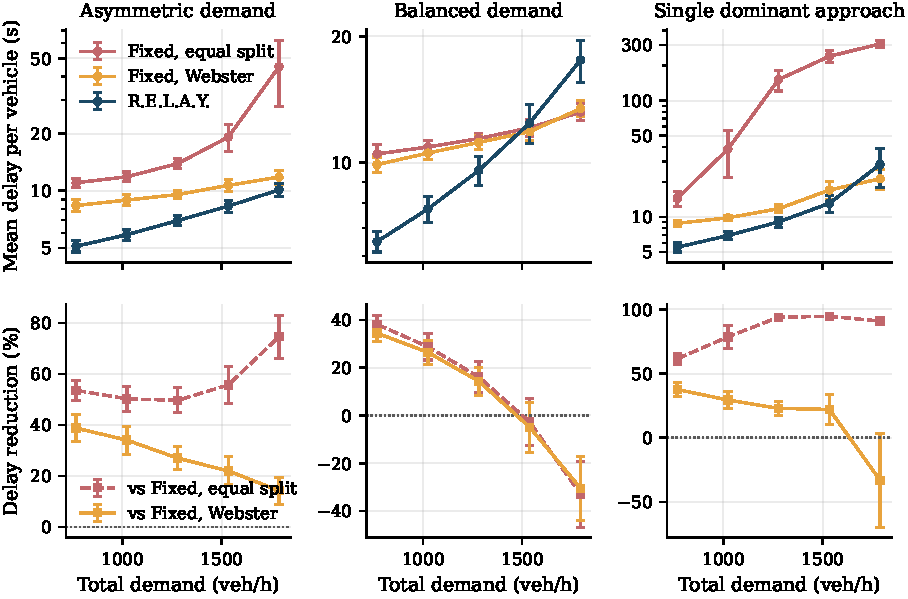
\includegraphics[width=\textwidth]{exp1_delay.pdf}
\caption{Experiment 1. Top row: mean delay per vehicle against total demand for the three demand
profiles, on a logarithmic axis. Bottom row: paired per-seed delay reduction achieved by \relay{}
against each fixed-time baseline. Error bars are one standard deviation across 30 seeds. Every cell
lies above zero against both baselines.}
\label{fig:exp1}
\end{figure}

\begin{figure}[t]
\centering
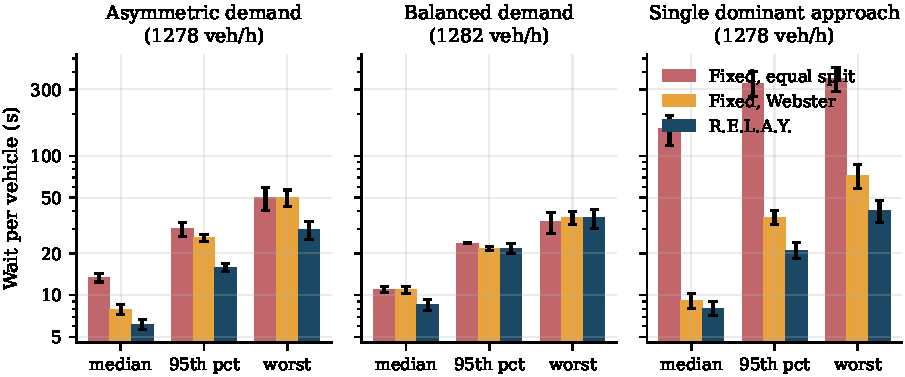
\includegraphics[width=\textwidth]{exp1_tail.pdf}
\caption{Experiment 1. Median, 95th-percentile and worst observed wait per vehicle at demand
multiplier 1.0, on a logarithmic axis. The tail, not the mean, is where the anti-starvation bound
shows: under a single dominant approach the equal-split plan's worst wait averages 361.5~s against
36.9~s for \relay.}
\label{fig:exp1tail}
\end{figure}

Figure~\ref{fig:exp1tail} shows the wait distribution rather than the mean, which is where the fairness
bound becomes visible. At 1278~veh/h under asymmetric demand the 95th-percentile wait is 29.9~s under
the equal-split plan, 25.8~s under the Webster plan and 14.5~s under \relay, with worst observed waits
averaging 50.0~s, 50.1~s and 26.7~s. Under a single dominant approach the contrast is larger: 333.4~s
and 36.3~s at the 95th percentile against 17.0~s under \relay, and worst waits of 361.5~s and 72.9~s
against 36.9~s, consistent with the forced-service rule at $R = 60$~s. The tail improves in every cell,
which matters more than the mean for a policy whose fairness claim is a bound rather than an average.
Figure~\ref{fig:exp1paired} shows the same comparison unaggregated, one point per seed.

\begin{figure}[t]
\centering
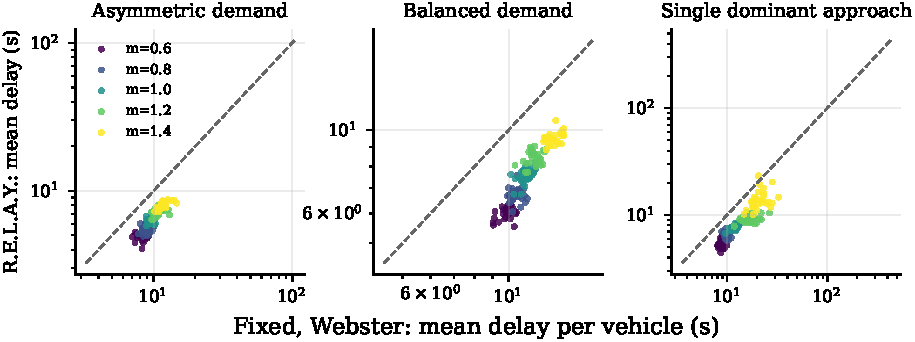
\includegraphics[width=\textwidth]{exp1_paired.pdf}
\caption{Experiment 1, unaggregated. Each point is one seed at one demand level, plotting \relay's
mean delay against the Webster plan's mean delay on the identical arrival stream. Points below the
diagonal favour \relay. Colour encodes the demand multiplier from 0.6 (dark) to 1.4 (light).}
\label{fig:exp1paired}
\end{figure}

\subsection{Switching, clearance, and what saturation costs an unconstrained policy}
\label{sec:discussion}

\begin{figure}[t]
\centering
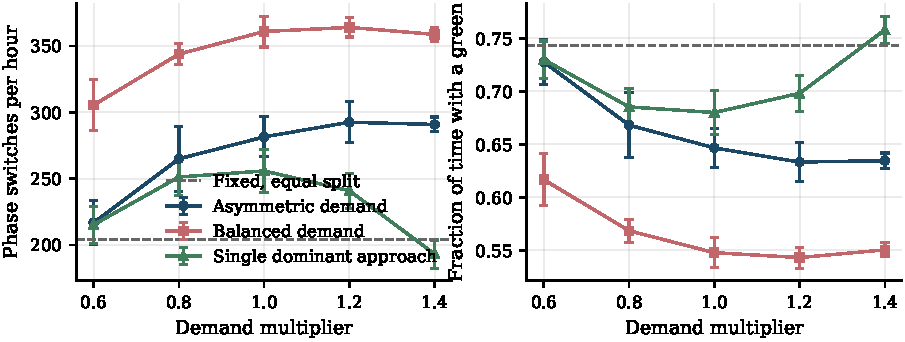
\includegraphics[width=\textwidth]{exp1b_switching.pdf}
\caption{Experiment 1b. Left: phase changes per hour. Right: the fraction of wall time during which
a green is displayed, the complement of which is time spent in yellow and all-red clearance. The
dashed line is the equal-split fixed plan, whose behaviour is independent of demand by construction.}
\label{fig:exp1b}
\end{figure}

Balanced saturated demand is where an unconstrained pressure policy fails, and the failure is worth
stating precisely because it motivates three of the rules in Section~\ref{sec:control}. No phase
dominates, so successive scores sit near-tied and any per-step comparison flips on noise. A constant
hysteresis margin is crossed almost immediately. The anti-starvation rule, if it fires whenever any
approach has waited past $R$, fires on every step, because beyond capacity every approach is past $R$
permanently. Both terminate green at $g_{\min}$, and the junction is no longer being controlled, only
alternated. Measured on this junction at 2307~veh/h, a policy with those two properties displays
5.2~s of green per 4.5~s of clearance interval, holds green for 0.54 of wall time against the fixed
plan's 0.80, and reaches 94~s of mean delay against that plan's 19~s.

This is the practical form of a known theoretical issue: max-pressure as formulated in the literature
evaluates its argmax freely and imposes no cycle structure, and Levin et al.
\citep{Levin2020CyclicalMaxPressure} propose a cyclical structure to recover the lost capacity.
Sections~\ref{sec:floor} and~\ref{sec:cost} recover it with a cycle measured rather than configured,
and the starvation rule of Section~\ref{sec:control} serves the worst-treated queue instead of
rotating among equally starved ones. Each is separately necessary; none requires a site survey.

Figure~\ref{fig:exp1b} shows what the resulting policy does. \relay{} switches more often than the
fixed plan under balanced demand, 282 to 331 per hour against 204, and displays green for less of the
wall clock, 0.585 to 0.646 against 0.743, while reducing delay by 28.4\% to 38.5\%. Displayed green
time is therefore not the objective: a fixed plan spends its green where the demand is not, and
slightly less green in the right place beats more of it in the wrong one. Where both effects align
the margin is largest, and under a single dominant approach at $m = 1.4$ \relay{} switches less than
the fixed plan, 167 per hour against 204, and holds green longer, 0.791 against 0.743.

\subsection{Corridor}

\begin{table}[t]
\centering
\caption{Experiment 2. Three-junction corridor, mean over 20 seeds with standard deviation in
parentheses. Delay is total queueing delay per vehicle across all junctions traversed. Through travel
time is measured for the two arterial through routes only; free-flow traversal of the three links is
21.6~s. Emergency traversal is the single emergency vehicle released in each run, whose standard
deviation is zero for the fixed plans because those plans are deterministic.}
\label{tab:exp2}
\small
\begin{tabular}{llcccc}
\toprule
Demand & & Mean delay & Through travel & Stops per & Emergency \\
(veh/h) & Policy & per vehicle (s) & time (s) & vehicle & traversal (s) \\
\midrule
769 & Webster, independent   & 26.7 (0.9) & 39.7 (0.9) & 1.95 & 36.0 (0.0) \\
    & Webster, coordinated   & 25.7 (0.7) & 37.0 (0.7) & 1.78 & 24.5 (0.0) \\
    & \relay, no coupling    & 11.3 (0.5) & 24.9 (0.5) & 1.09 & 22.3 (3.3) \\
    & \relay, coupled        & 11.2 (0.5) & 24.9 (0.5) & 1.09 & 22.3 (3.3) \\
\midrule
1282& Webster, independent   & 30.1 (0.8) & 41.5 (0.7) & 2.09 & 53.6 (7.5) \\
    & Webster, coordinated   & 29.2 (1.1) & 38.0 (0.8) & 1.80 & 31.5 (0.0) \\
    & \relay, no coupling    & 15.2 (0.7) & 28.3 (0.6) & 1.53 & 23.7 (4.7) \\
    & \relay, coupled        & 15.2 (0.6) & 28.5 (0.6) & 1.53 & 24.2 (6.7) \\
\midrule
1794& Webster, independent   & 36.7 (3.3) & 43.1 (1.3) & 2.10 & 30.1 (6.5) \\
    & Webster, coordinated   & 35.3 (3.6) & 39.3 (0.9) & 2.03 & 24.0 (0.0) \\
    & \relay, no coupling    & 20.0 (0.8) & 31.9 (0.5) & 1.86 & 26.1 (8.5) \\
    & \relay, coupled        & 20.2 (0.8) & 32.4 (0.7) & 1.86 & 27.6 (8.2) \\
\bottomrule
\end{tabular}
\end{table}

\begin{figure}[t]
\centering
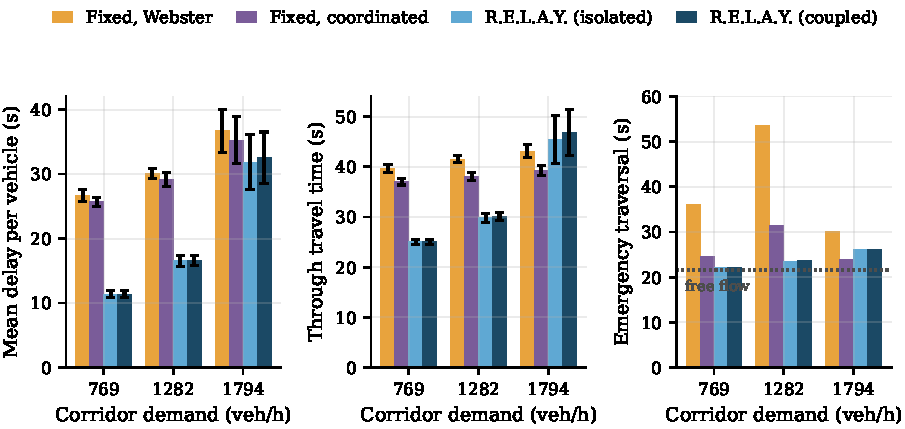
\includegraphics[width=\textwidth]{exp2_corridor.pdf}
\caption{Experiment 2. Left: mean queueing delay per vehicle across the corridor. Centre: travel
time for the two arterial through routes, where both adaptive variants stay below the coordinated
fixed plan at every demand level. Right: traversal time of the single emergency vehicle released in
each run, against the 21.6~s free-flow reference.}
\label{fig:exp2}
\end{figure}

Table~\ref{tab:exp2} and Figure~\ref{fig:exp2} contain three findings, one of them negative.

First, the delay reduction is large across the range and decays only gradually with demand: 57.9\%,
49.4\% and 44.6\% against the independent Webster plans at 769, 1282 and 1794~veh/h, and 56.3\%,
47.8\% and 42.2\% against the coordinated plan. The coordinated plan is only 2 to 4\% better than the
independent plans on mean delay, as expected, since progression offsets improve the through movement
and not the average over all movements. Arterial through travel time and stops per vehicle improve
together with delay: at the highest demand, 32.4~s and 1.86 stops against the coordinated plan's
39.3~s and 2.03, so the gain is not obtained by trading progression for total delay.

Second, the coupling term does essentially nothing. Disabling it, which turns the corridor into three
independently adaptive junctions, changes mean delay by $+0.1\%$, $-0.5\%$ and $-0.9\%$ at the three
demand levels, and at the two higher levels the uncoupled variant is marginally better. The corridor
benefit is therefore attributable to local adaptivity, not to coordination. We report this plainly
because the coupling term is part of the system's design rationale and the data do not support it.
Two explanations are consistent with our setup and we cannot separate them here: the point-queue
model has no spatial extent, so a downstream queue never physically blocks an upstream discharge,
which removes the main mechanism the coupling addresses; and a single aggregate downstream queue is a
weak proxy for the movement-specific pressure difference max-pressure theory uses. Distinguishing
them requires a model with link storage, which we regard as the most informative single extension to
this evaluation.

Third, the emergency result is unambiguous. The emergency vehicle traverses the corridor in 22.3 to
27.6~s under \relay{} against a free-flow reference of 21.6~s, so it is delayed by roughly 1 to 6~s
across three signalised junctions, against 30.1 to 53.6~s under the independent Webster plans. The
coordinated plan does well here, 24.0 to 31.5~s, because the emergency vehicle travels in the
progression direction; a westbound emergency would not benefit, whereas \relay{} is direction-agnostic
by construction.

\subsection{Emergency preemption latency}

\begin{table}[t]
\centering
\caption{Experiment 3. Delay from the first emergency detection to green on the emergency approach,
over 900 trials. The equal-split baseline has no preemption path, so its latency is determined by
cycle position and is independent of demand, which is why its statistics are pooled.}
\label{tab:exp3}
\small
\begin{tabular}{lcccccc}
\toprule
Demand & Policy & Mean (s) & SD (s) & Median (s) & 95th pct (s) & Worst (s) \\
\midrule
Light ($m{=}0.6$)  & \relay{} & 4.01 & 3.55 & 4.58 & 10.77 & 13.61 \\
Medium ($m{=}1.0$) & \relay{} & 4.06 & 3.90 & 4.31 & 11.88 & 13.91 \\
Heavy ($m{=}1.4$)  & \relay{} & 4.19 & 3.89 & 4.54 & 11.85 & 13.99 \\
All                & \relay{} & 4.09 & 3.78 & 4.54 & 11.33 & 13.99 \\
All                & Equal split & 7.00 & 7.04 & 5.02 & 20.59 & 22.29 \\
\bottomrule
\end{tabular}
\end{table}

\begin{figure}[t]
\centering
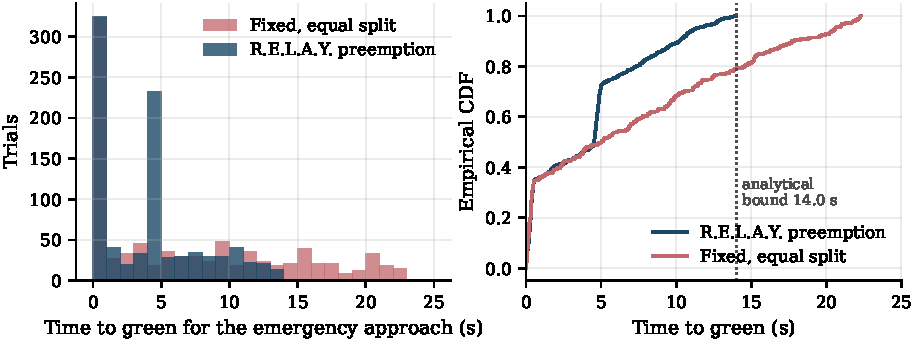
\includegraphics[width=\textwidth]{exp3_preemption.pdf}
\caption{Experiment 3. Left: histogram of the time from the first emergency detection to green on the
emergency approach, over 900 trials. Right: the same data as empirical cumulative distributions
against the analytical bound of Equation~\eqref{eq:bound}.}
\label{fig:exp3}
\end{figure}

Mean latency is 4.09~s against 7.00~s for the fixed cycle, and is almost insensitive to demand, rising
only from 4.01~s to 4.19~s between the lightest and heaviest loads (Table~\ref{tab:exp3}). That
insensitivity is a design property rather than a coincidence: the green allocated by
Equation~\ref{eq:floor} grows with saturation, but preemption is evaluated above it against
$g_{\min}$, so a busier junction does not make an emergency vehicle wait longer. The important
quantity is the tail: the 95th percentile is 11.33~s against 20.59~s and the worst case over 900
trials is 13.99~s against 22.29~s. The measured worst case sits 0.01~s below the analytical bound of 14.0~s
from Equation~\eqref{eq:bound}, and inspecting the worst trials confirms the predicted mechanism, since
every trial above 13.4~s is one in which the announcement arrived within the first second of a yellow
already transitioning away from the emergency's own phase. Because the bound is composed only of
clearance and minimum-green settings, it can be tightened by configuration and stated in advance to an
emergency service, which a demand-blind fixed plan cannot do.

Two qualifications belong with this result. In 311 of 900 trials, or 34.6\%, the emergency approach
already had green when the vehicle was detected, so latency was effectively zero and the mean is pulled
down accordingly; and in 298 trials, or 33.1\%, the fixed cycle happened to reach that approach sooner
than the preemption did, which is why the distributions overlap substantially in
Figure~\ref{fig:exp3} even though tail behaviour differs sharply. The claim these data support is a
bounded worst case, not a uniformly faster response.

\subsection{Perception}
\label{sec:perception}

\begin{table}[t]
\centering
\caption{Experiment 4. Detector performance on the system's held-out split: 97 images, 4990 labelled
instances. The checkpoint evaluated is the one shipped with the system, a 2.59-million parameter
model. P and R are precision and recall at the operating point the validator reports.}
\label{tab:detector}
\footnotesize
\setlength{\tabcolsep}{4.5pt}
\begin{tabular}{lccccccccc}
\toprule
& \multicolumn{4}{c}{Overall} & \multicolumn{5}{c}{AP@50 by class} \\
\cmidrule(lr){2-5}\cmidrule(lr){6-10}
Model & mAP@50 & mAP@50-95 & P & R & car & motorcycle & bus & truck & ambulance \\
\midrule
Shipped fine-tune & 0.954 & 0.809 & 0.950 & 0.886 & 0.985 & 0.851 & 0.981 & 0.964 & 0.987 \\
\bottomrule
\end{tabular}
\end{table}

\begin{figure}[t]
\centering
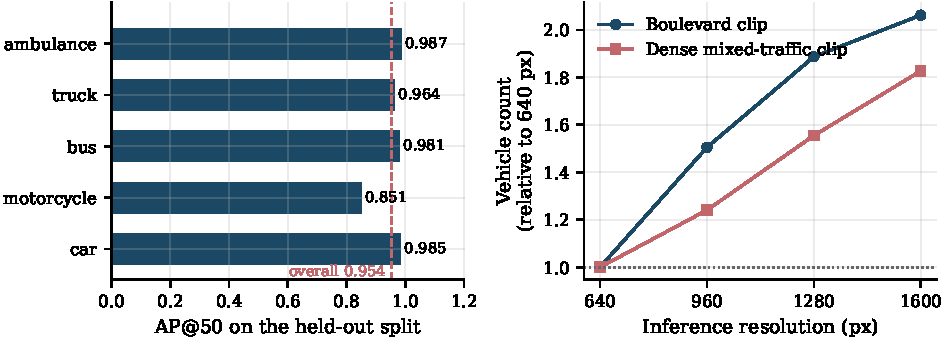
\includegraphics[width=\textwidth]{detector.pdf}
\caption{Experiment 4. Left: per-class average precision at IoU 0.5 on the held-out split, with the
overall mean average precision marked. Right: sampled vehicle count as a function of inference
resolution, normalised to the count at 640~px. Neither curve has flattened by 1600~px, which is
direct evidence that vehicles are still being missed.}
\label{fig:detector}
\end{figure}

Table~\ref{tab:detector} reports mean average precision of 0.954 at IoU 0.5 and 0.809 averaged over
IoU 0.5 to 0.95, with precision 0.950 and recall 0.886. Per-class average precision exceeds 0.96 for
cars, buses, trucks and ambulances and is lowest for motorcycles at 0.851, the expected ordering given
that two-wheelers are the smallest and most frequently occluded class. An important caveat concerns what
the split is: it mixes automatically labelled frames from a synthetic feed with frames from real footage
pseudo-labelled by a general detector rather than by human annotation, so a high score establishes that
the fine-tuned model reproduces the labelling function it was trained against, not accuracy against human
ground truth, and the ambulance figure of 0.987 reflects a class that is easy to separate in the synthetic
domain. We deliberately omit a comparison against general COCO-trained checkpoints on this split, because
their class indices do not correspond to this label space and any such comparison would be an artefact of
index mismatch.

Running the full perception stack on real footage at 960~px inference on an Apple M3 Pro, median
per-frame latency is 38.3~ms on the boulevard clip (26.1 frames per second, 95th percentile 85.7~ms) and
85.8~ms on the dense mixed-traffic clip (11.7 frames per second, 95th percentile 130.7~ms); the first
frame of a run costs 1735~ms because of one-off backend initialisation and is excluded. Both rates exceed
what the control loop needs, since decision epochs are governed by the 5~s minimum green rather than by
the frame rate, and perception is decoupled from control so a latency spike delays a count update rather
than blocking a decision.

\begin{figure}[t]
\centering
\begin{subfigure}{\textwidth}
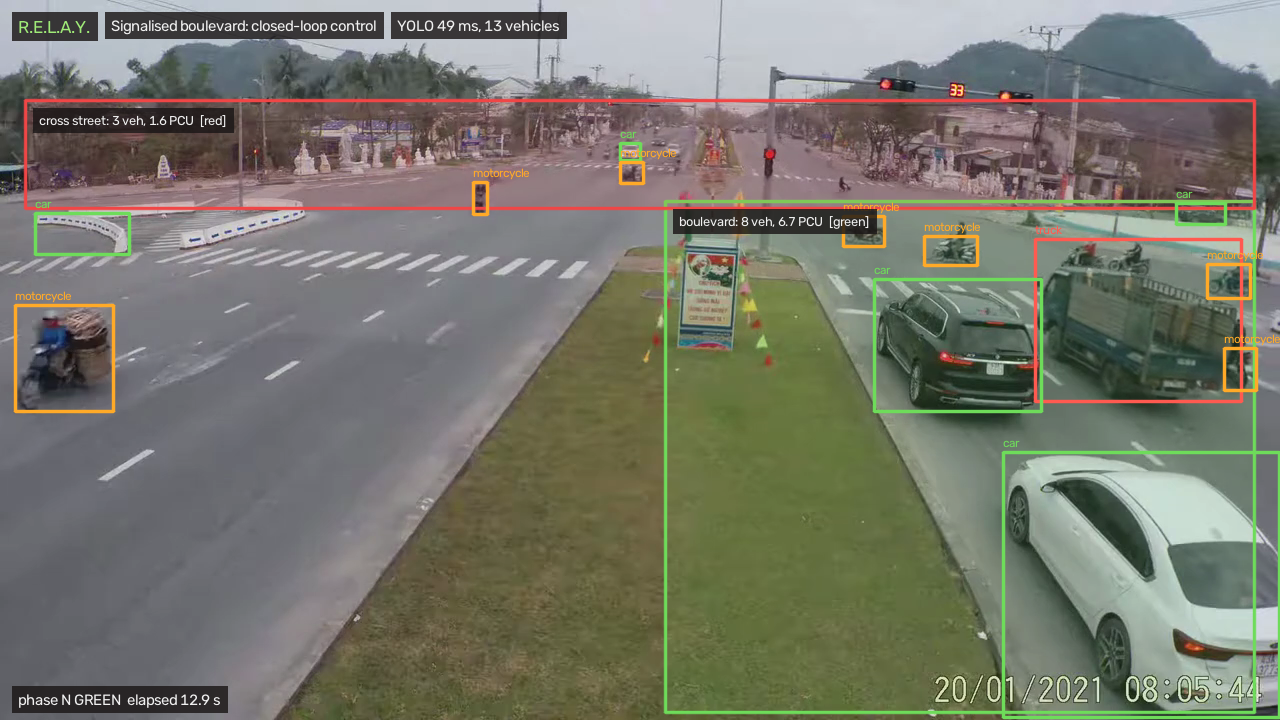
\includegraphics[width=\textwidth]{frame_levanhien_22s.png}
\caption{Signalised boulevard. The controller is running on these counts: the near boulevard approach
holds 8 vehicles and 6.7~\pcu{} and has green, the crossing street holds 3 vehicles and 1.6~\pcu{}
and is red, and the header reports the real inference latency for the frame.}
\end{subfigure}
\vspace{0.5em}
\begin{subfigure}{\textwidth}
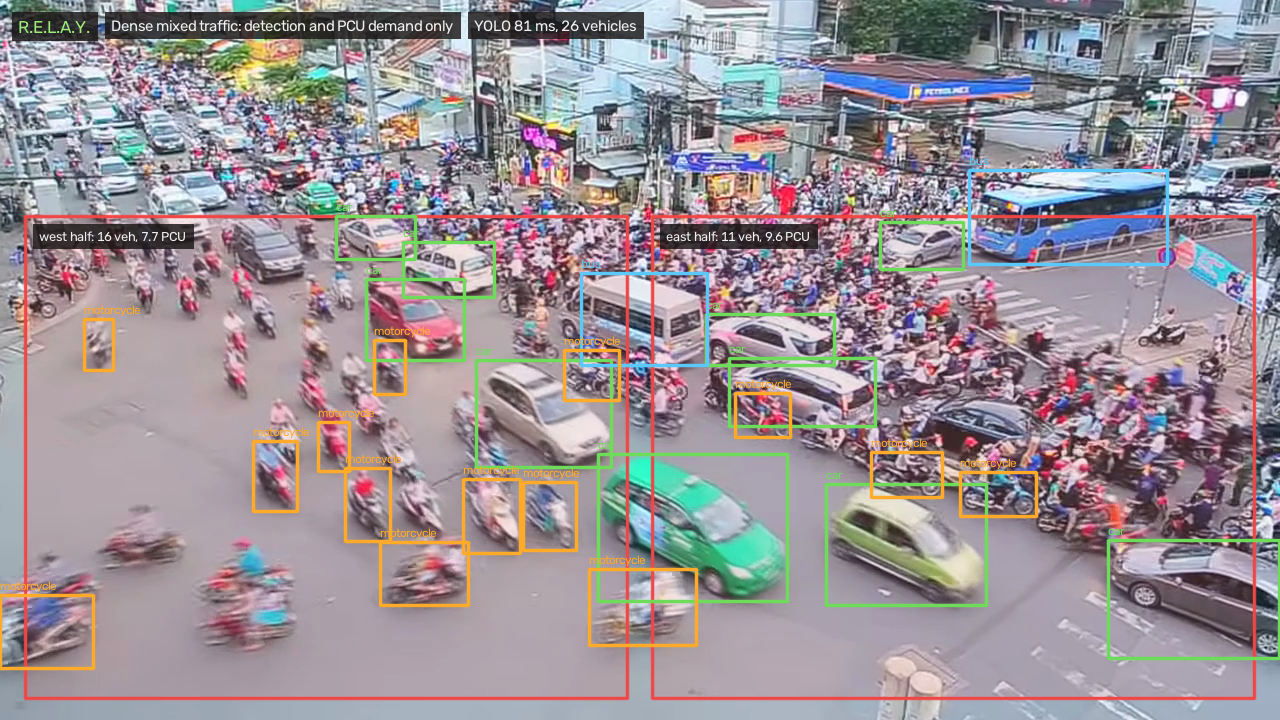
\includegraphics[width=\textwidth]{frame_hcmc_18s.png}
\caption{Dense motorcycle-dominated traffic. The failure mode is visible: 26 vehicles are detected in
a scene containing several hundred, so the reported \pcu{} demand of 7.7 and 9.6 for the two halves
is a severe underestimate. No controller decision is shown, because the junction depicted is not
signal-controlled in the way the two zones imply.}
\end{subfigure}
\caption{Experiment 4. The perception stack on real fixed-camera footage. Both frames are direct
output of the system, with detections, approach polygons and per-approach \pcu{} demand as computed
at run time.}
\label{fig:frames}
\end{figure}

Figure~\ref{fig:frames} shows annotated frames from both clips, and the second shows the main
perception weakness plainly. To quantify rather than assert it, we measured how the count changes with
inference resolution (Figure~\ref{fig:detector}, right). On the dense clip the mean sampled vehicle
count rises from 21.4 at 640~px to 26.5 at 960~px, 33.2 at 1280~px and 39.1 at 1600~px, an increase of
83\% with no sign of convergence, and motorcycles alone rise by 120\%; on the sparser boulevard clip
the count rises from 4.85 to 10.0. A count that keeps growing with resolution has not converged, so the
absolute demand values the controller receives on dense two-wheeler scenes are underestimates of
unknown magnitude. Median inference cost over the same range rises from 47.2~ms to 108.0~ms, so raising
resolution is not free.

This weakness does not immediately invalidate the control results, because the controller compares
approaches rather than reading absolute volumes, so a systematic undercount affecting both approaches
similarly leaves the ordering of phase scores intact. What it does affect is any rule keyed to an
absolute quantity, in particular the occupancy indicator $o_a$ near an empty approach and the gap-out
timer. A regionally fine-tuned detector on human-annotated South Asian footage is the direct remedy and
is not attempted here.

Taken together, these results support a narrower claim than the one usually made for camera-based adaptive
control. The controller helps most where demand is imbalanced and the junction is not saturated, and its
operational value is clearest in the bounds rather than the means: the worst observed wait tracks the
configured $R$ across every profile and the preemption worst case is bounded in closed form, so an
authority can be told in advance what the guarantees are. The coordination term is not supported by our
data, and the pedestrian logic, though verified by executable invariants, was never benchmarked against a
pedestrian-aware baseline, so we claim no pedestrian delay benefit.

\subsection{Robustness across demand shapes and topology}
\label{sec:robustness}

\begin{table}[t]
\centering
\caption{Experiment 6. Worst and median paired delay reduction over the eight load levels of each
demand shape, 25 seeds per cell. Positive favours \relay. The worst column is the reportable one:
an adaptive policy that wins on average and loses at one shape is not deployable.}
\label{tab:exp6}
\small
\begin{tabular}{llccc}
\toprule
Topology & Demand shape & Worst vs equal (\%) & Worst vs Webster (\%) & Median vs Webster (\%) \\
\midrule
Four-way & Asymmetric   & $+53.3$ & $+29.2$ & $+34.4$ \\
         & Balanced     & $+27.1$ & $+27.0$ & $+32.5$ \\
         & Near-equal   & $+28.5$ & $+27.9$ & $+33.0$ \\
         & One axis     & $+63.4$ & $+29.3$ & $+38.8$ \\
         & Three heavy  & $+33.1$ & $+34.3$ & $+36.0$ \\
         & Lopsided     & $+52.6$ & $+30.5$ & $+34.8$ \\
         & Single       & $+61.3$ & $-26.6$ & $+38.5$ \\
\midrule
T-junction & Balanced   & $+37.1$ & $+37.0$ & $+39.6$ \\
           & Arterial   & $+63.1$ & $+30.5$ & $+40.6$ \\
\bottomrule
\end{tabular}
\end{table}

Table~\ref{tab:exp6} reports the wider grid. \relay{} reduces mean delay against both fixed-time
baselines in 71 of 72 cells, spanning 432 to 2462~veh/h, and never falls below $+26.1\%$ against the
equal-split plan anywhere in the grid.

The single exception is the single-dominant-approach shape at the highest load, where the dominant
approach alone demands 1620~veh/h against a saturation flow of 1980~veh/h, or 82\% of all displayed
green. Balancing that against the 9~s of lost time a two-stage cycle costs requires a cycle of at
least 134~s, which is longer than the 60~s fairness bound $R$ configured for these runs permits. The
Webster reference is not subject to that constraint: it is granted a 120~s cycle and holds the minor
approach on red for 107~s, and it is itself unstable there, with a residual queue at the end of the
measurement window. Throughput is close to parity, 2222 against 2238~veh/h, and \relay's mean delay is
26.6\% higher. The honest description is that neither controller serves this demand, and that the
comparison rewards the one that abandons the fairness bound. An operator who
wants the Webster allocation here can have it by raising $R$; that is a policy decision about how long
a minor approach may be held, not a control-law result, and we do not report it as a win.

Repeating the entire grid with 20\% zero-mean Gaussian miscounting on every count the controller sees
leaves the picture unchanged: 71 of 72 cells still win, the worst cell against the equal-split plan
moves from $+27.1\%$ to $+26.1\%$, and the same single cell is the exception. The estimators of
Section~\ref{sec:estimation} smooth over a $\tau = 60$~s window, which is long relative to the noise,
and the decisions they feed are floors and margins rather than instantaneous set points.

That test is the easy one. A zero-mean error averages out over the smoothing window by
construction, whereas Section~\ref{sec:perception} measures a \emph{biased} one: the detector
reports 26 vehicles in a scene holding several hundred, and counts still climb 83\% between 640~px
and 1600~px without converging. We therefore repeat the grid under two count models that are wrong
in the direction the detector is wrong. Queues stay exact in both, so what is measured is the
control response to a wrong observation.

The first saturates, $\hat q = q/(1 + q/C)$: near-exact on a light approach, increasingly short as
it fills, which is the shape of the measured failure. At $C = 15$ and $C = 30$ the result is
unchanged, 71 of 72 cells, worst margin $+26.6\%$ against the equal-split plan, and a mean cost
across the grid of $-0.3$ percentage points. The largest single-cell loss is 1.6 points. Saturation
preserves the ordering of approaches and stays accurate where the estimators work, distorting only
a tail that was going to be served anyway. The one cell the controller loses improves under it,
from $-26.6\%$ to $-4.2\%$, because compressing the dominant approach's count stops the policy
contending against the fairness bound.

The second is a flat multiplicative loss, $\hat q = \lfloor \kappa q \rceil$. Down to $\kappa = 0.6$
it costs nothing measurable: 71 of 72 cells at $\kappa = 0.9$, $0.8$, $0.7$ and $0.6$, mean cost at
most $0.1$ points. That is a property of the formulation, not a lucky range. The degree of
saturation in Section~\ref{sec:floor} is a ratio of an arrival estimate to a discharge estimate
drawn from the same counts, so a uniform scale factor cancels before it reaches a decision.

At $\kappa = 0.5$ the controller collapses to 50 of 72 cells and a mean cost of 32.7 points, behind
even the equal-split plan in the worst cell ($-11.1\%$). The discontinuity is not a magnitude
effect. At $\kappa = 0.5$ a lone vehicle rounds to zero, an occupied approach reports empty, and
empty-phase skipping declines to serve it; at $\kappa = 0.6$ it survives rounding. Repeating
$\kappa = 0.5$ with the single change that an occupied approach may never report empty restores the
result completely: 71 of 72 cells, worst margin $+26.4\%$, mean cost 0.2 points. The 50\% magnitude
error was never the problem.

The requirement this yields is narrower and more testable than "the detector must be accurate".
What the controller needs is an unbiased \emph{presence} signal at short queue lengths, not an
accurate absolute count. A detector that undercounts a crowd by an order of magnitude is tolerable,
because both the pressure ordering and the saturation ratio survive it; one that cannot separate an
empty approach from a nearly empty one is not, whatever its aggregate accuracy. That is a condition
a field trial can check on a candidate detector before a signal is connected to it, and it is one
the stack of Section~\ref{sec:perception} has not been shown to meet.

\section{Limitations}
\label{sec:limitations}

We list the limitations we believe would most affect a reader's assessment, in descending order of
importance.

\textbf{This is not a field study.} No signal was controlled. There is no controller cabinet in the loop,
no communication with a real signal and no before-and-after measurement, so we have no evidence about the
failure modes that appear only in the field: power interruption, lens contamination, camera
repositioning, seasonal light changes, or the behaviour of drivers who learn that the signal responds to
them. Every quantitative claim should be read with that scope.

\textbf{The traffic model is a point queue.} Queues have no spatial extent, so there is no spillback, no
blocking of an upstream junction by a downstream queue, no lane changing and no capacity loss from
vehicles obstructing the junction box. The abstraction is favourable to any adaptive policy, whose
mistakes are cheaper when queues cannot physically block anything, and specifically unfavourable to our
coordination term, whose purpose is to prevent a jam being fed, so the corridor coupling result should be
read as inconclusive rather than negative and a spatially explicit model in SUMO
\citep{lopez2018microscopic} would settle it.

\textbf{Perception was neither validated against human ground truth nor propagated into the control
experiments.} The held-out split mixes synthetic frames with pseudo-labelled real frames, so the
reported mean average precision of 0.954 measures agreement with the labelling process rather than
accuracy against human annotation; we can state that counts on dense footage are underestimates that have
not converged by 1600~px inference, but not the error magnitude, and a human-annotated evaluation set from
the target city is required before any absolute demand claim. Experiment 6 addresses only part of the
consequence: it shows the control policy tolerates 20\% zero-mean miscounting, but real detector error is
neither zero-mean nor independent across approaches, and undercounting two-wheelers biases whole phases in
one direction, which a symmetric noise model cannot reproduce. Measuring how much of the delay reduction
survives the detector's actual, structured error remains the most important open question for the design.

\textbf{The \pcu{} weights are configuration, not calibration.} The values in Table~\ref{tab:pcu} were
chosen to reflect a motorcycle-dominated mix rather than estimated from local field measurements.
Because they directly scale the pressure in Equation~\eqref{eq:vehpressure}, a mis-specified motorcycle
weight biases every phase comparison at a junction whose approaches differ in class mixture, and we ran
no sensitivity analysis over them.

\textbf{The loop is never closed.} Control results come from simulated counts and perception
results from recorded footage, and at no point in this work does the detector drive the controller.
The two halves are evaluated against each other only through the count-error models of
Section~\ref{sec:robustness}, which is an argument about robustness rather than a demonstration of
the assembled system. Those models are chosen to match the error the detector measurably makes and
the controller survives them, but a genuine end-to-end run, detector to signal head on the same
footage, is the obvious next experiment and it is not in this paper.

\textbf{Four narrower gaps.} The evaluated junctions have two stages, so although the controller
generates movement-level phasing and protected-left stages, the results do not exercise them; a junction
with five or six stages carries proportionally more lost time per cycle, and while
Equation~\ref{eq:floor} lengthens the cycle in response, we have not measured whether it does so
correctly when the disjoint cover has more than two members. We compare only against fixed-time plans,
whereas the natural research baseline for a pressure-based controller is a learned policy, PressLight
\citep{wei2019presslight} in particular since its reward derives from max-pressure; our reasons for not
deploying one are practical and stated in Section~2, but they do not excuse the absence of a comparison
that would locate this controller between fixed-time and learned control. The pedestrian logic is
asserted by executable invariants but never compared against an alternative treatment such as a
conventional fixed pedestrian stage, so we report its behaviour and not its benefit. Finally, the
fairness bound $R$ is the parameter the results are most sensitive to: Section~\ref{sec:robustness}
shows it, and not the pressure rule, decides the one cell where a fixed plan wins, and we have not
characterised the delay-fairness frontier it traces.

\section{Conclusion}

We have described a single-camera adaptive signal controller for heterogeneous urban traffic and
evaluated it in a seeded microsimulation and on real fixed-camera footage. The controller converts
per-approach, per-class detections into \pcu-weighted demand and selects phases by a queue-weighted
pressure score in the max-pressure family, with the operational rules a deployable signal requires:
clearance intervals, minimum and maximum green, empty-phase skipping, gap-out, a hard maximum-wait bound
for vehicles and a separate one for pedestrians, and emergency preemption with a bounded hold.

Its distinguishing feature is that it measures the junction rather than being told about it. Arrival and
discharge rates are estimated per approach from the same count sequence the detector already produces,
and they determine both the green each stage receives, through Webster's cycle evaluated on the measured
degree of saturation, and the margin a competing stage must clear, through the discharge that a clearance
interval forfeits. Both are what a plain argmax policy lacks: without them, an unconstrained pressure
rule terminates every green at the safety minimum once demand approaches capacity, spending the
junction's capacity on amber. Neither requires a traffic survey, a saturation-flow table, or any
per-site constant, which matters for a deployment context where those are exactly what is unavailable.

Measured against a fixed-time plan granted the true mean demand, the controller reduces mean delay in
every cell of both the primary grid and a wider 72-cell robustness grid but one, by 28.4\% to 44.3\% at a
single junction and 44.6\% to 57.9\% across a three-junction corridor, cuts the 95th-percentile and
worst-case waits proportionally further than it cuts the mean, and brings an emergency vehicle to green
within a worst case of 13.99~s against an analytical bound of 14.0~s. The single exception is an
approach demanding 82\% of all displayed green, where the configured fairness bound forbids a cycle long
enough to be stable and the fixed plan wins by not observing one.

One result is negative and reported rather than suppressed: the corridor coordination term produces no
measurable benefit in our model, changing mean delay by at most 0.9\%, so the corridor gain is
attributable to local adaptivity alone. The next steps follow from the limitations: a spatially explicit
corridor model to settle whether the coordination term is useful, a sensitivity study using the
detector's own structured error rather than symmetric noise, a human-annotated evaluation set from the
target city, and a field trial.

\section*{Data and code availability}

The controller, perception stack and simulation harness are available at
\url{https://github.com/kafle1/relay} under the AGPL-3.0 licence. The experiment scripts that
produced every table and figure, the raw per-run result files, the captured invariant-check output
and the figure generation script are distributed with this manuscript in the \texttt{experiments/}
directory. Re-running the experiment scripts and then the figure script reproduces every number and
every panel reported here. The reproduction is exact rather than statistical: every run is seeded,
and re-running Experiment 6 from a clean clone returns all 72 cells identical to the values reported
here. A checker, \texttt{experiments/verify\_claims.py}, reads the numerical claims out of this
manuscript and recomputes each one from the raw result files, so a figure quoted in the text and the
data behind it cannot drift apart unnoticed.

\section*{Declarations}

The author declares no competing interests and received no funding for this work. No human subjects
or personal data were involved: the footage used is publicly available recorded video of public
roads, used only for aggregate vehicle counting, and no identification of individuals or vehicles was
performed or attempted.

\bibliographystyle{unsrtnat}
\bibliography{refs}

\end{document}
